\documentclass[a4paper,UTF8]{ctexart}
\usepackage{graphicx}
\usepackage{geometry}
\usepackage{xcolor}
\usepackage{amsmath}
\usepackage{enumerate}
\usepackage{caption}
\usepackage{listings}
\usepackage{array}
\usepackage{booktabs}
\usepackage{tikz}
\usetikzlibrary{shapes,arrows}
% \usepackage{pgfplots}
% \pgfplotsset{compat=1.17}
\usepackage{appendix}
\captionsetup[lstlisting]{labelfont=bf,justification=justified}
\usepackage{multicol}
\setlength{\columnsep}{3em}
\usepackage{float}
\usepackage{circuitikz}
\usepackage{ulem}

\graphicspath{{img/}}

\usepackage[colorlinks,linkcolor=blue]{hyperref}
\usepackage{bookmark}
\providecommand{\code}[2]{\lstinputlisting[language=#2,caption=\href{run:#1}{\ttfamily #1}]{#1}}
\providecommand{\img}[1]{\includegraphics[width=0.88\textwidth]{#1}}

% listings
\definecolor{grey}{rgb}{0.8,0.8,0.8}
\definecolor{darkgreen}{rgb}{0,0.3,0}
\definecolor{darkblue}{rgb}{0,0,0.3}
\lstset{%
    numbers=left, %行号
    numberstyle=\scriptsize\color{grey},
    showstringspaces=false,
    showspaces=false,%
    tabsize=4,%
    frame=shadowbox,%
    basicstyle={\ttfamily\normalsize},%
    keywordstyle=\color{blue!80!black}\bfseries,%
    identifierstyle=,%
    commentstyle=\color{green!50!blue}\itshape,%
    stringstyle=\color{green!50!black},%
    rulesepcolor=\color{gray!20!white},
    breaklines,
    columns=flexible,
    extendedchars=false,
    %mathescape=true,
    language=verilog,
}

\begin{document}
\title{\normalsize \underline{计算机系统结构实验}\\\LARGE 实验 6 报告\\\vspace*{1em}\normalsize 类MIPS多周期流水线处理器的设计与实现}
\author{李子龙\\ 518070910095}
\date{\today}
\maketitle
\tableofcontents
\clearpage

\section{实验目的}

\begin{enumerate}
    \item 理解CPU Pipeline,了解流水线冒险(hazard)及相关性,设计基础流水线CPU
    \item 增加Forwarding机制解决数据竞争,减少因数据竞争带来的流水线停顿延时,提高流水线处理器性能
    \item 设计支持Stall的流水线CPU。通过检测竞争并插入停顿(Stall)机制解决数据冒险、控制竞争和结构冒险
    \item 通过predict-not-taken或延时转移策略解决控制冒险/竞争,减少控制竞争带来的流水线停顿延时,进一步提高处理器性能
    \item \sout{将CPU支持的指令数量从16条扩充为31条,使处理器功能更加丰富(选做)}
\end{enumerate}

\section{原理分析}

\subsection{基础流水线}
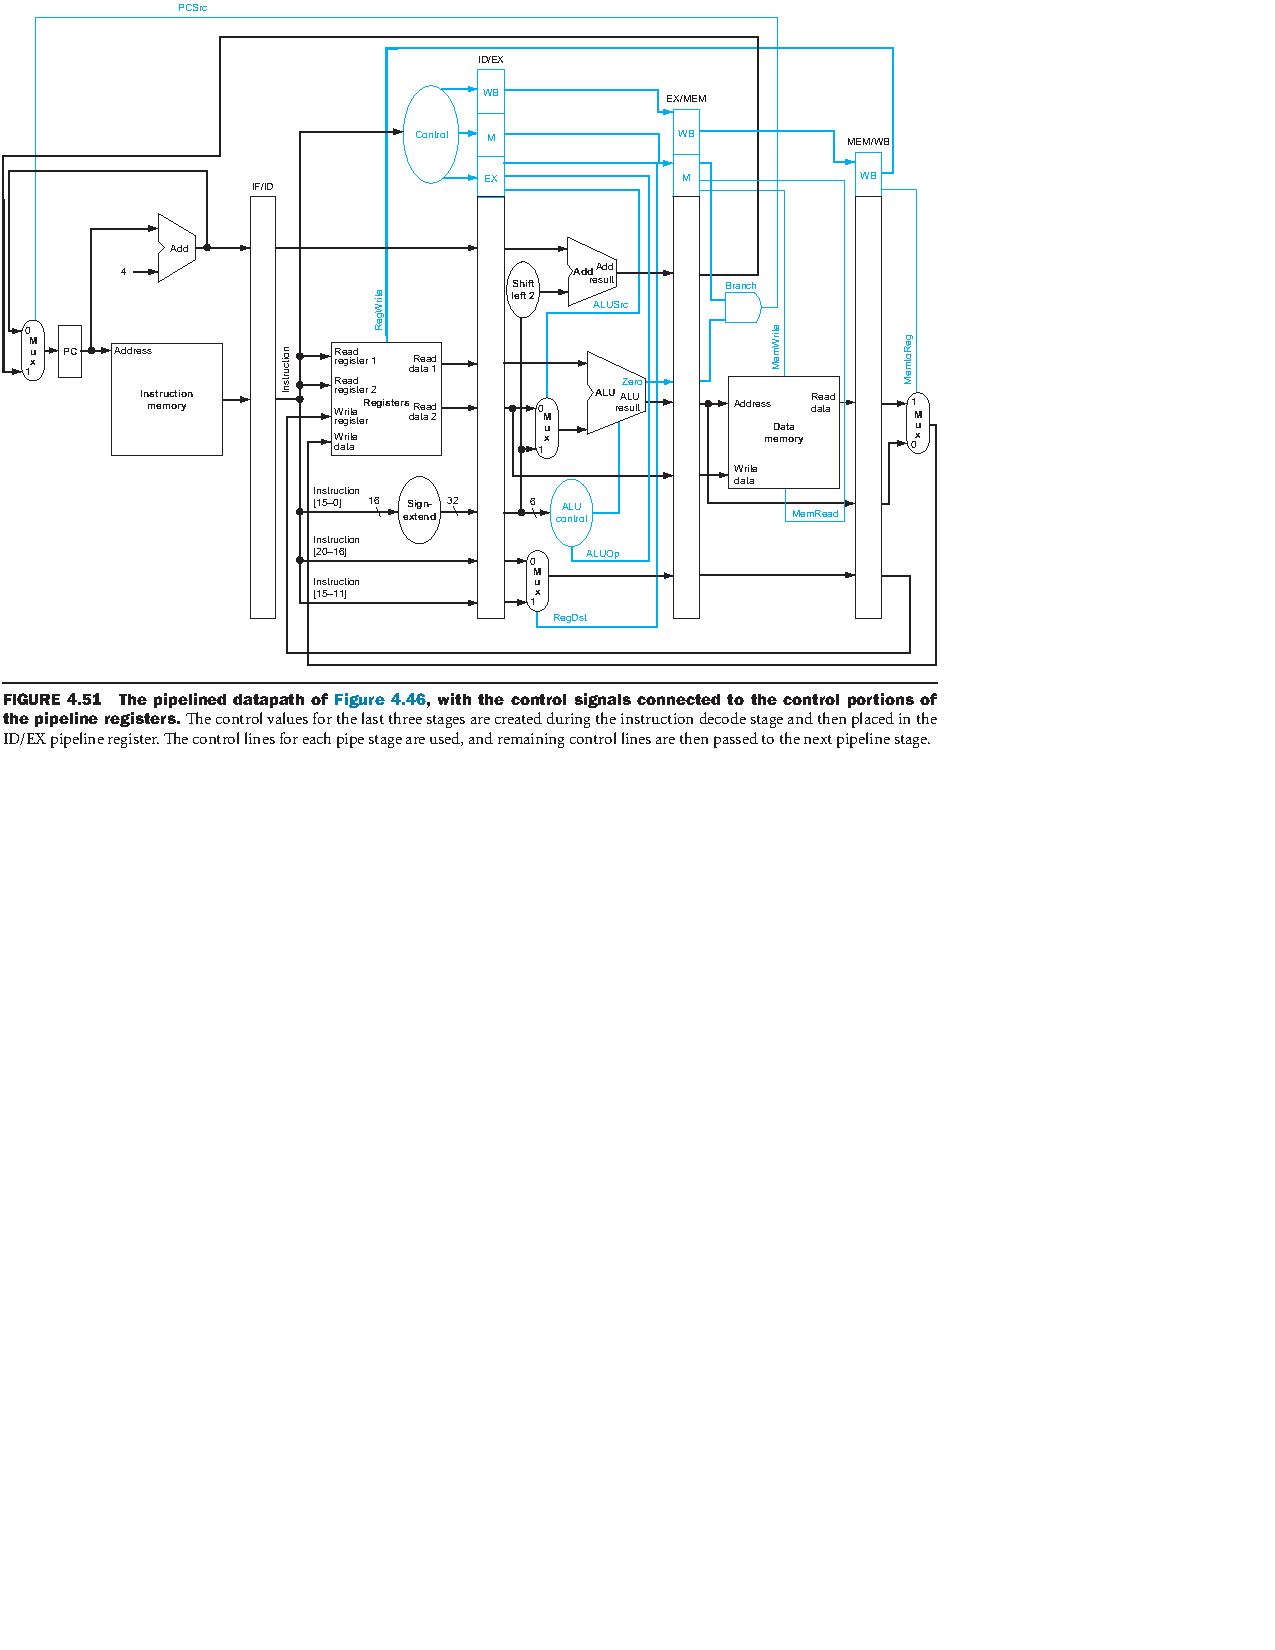
\includegraphics[width=\textwidth]{pipeline.pdf}



\subsection{前向转发机制}
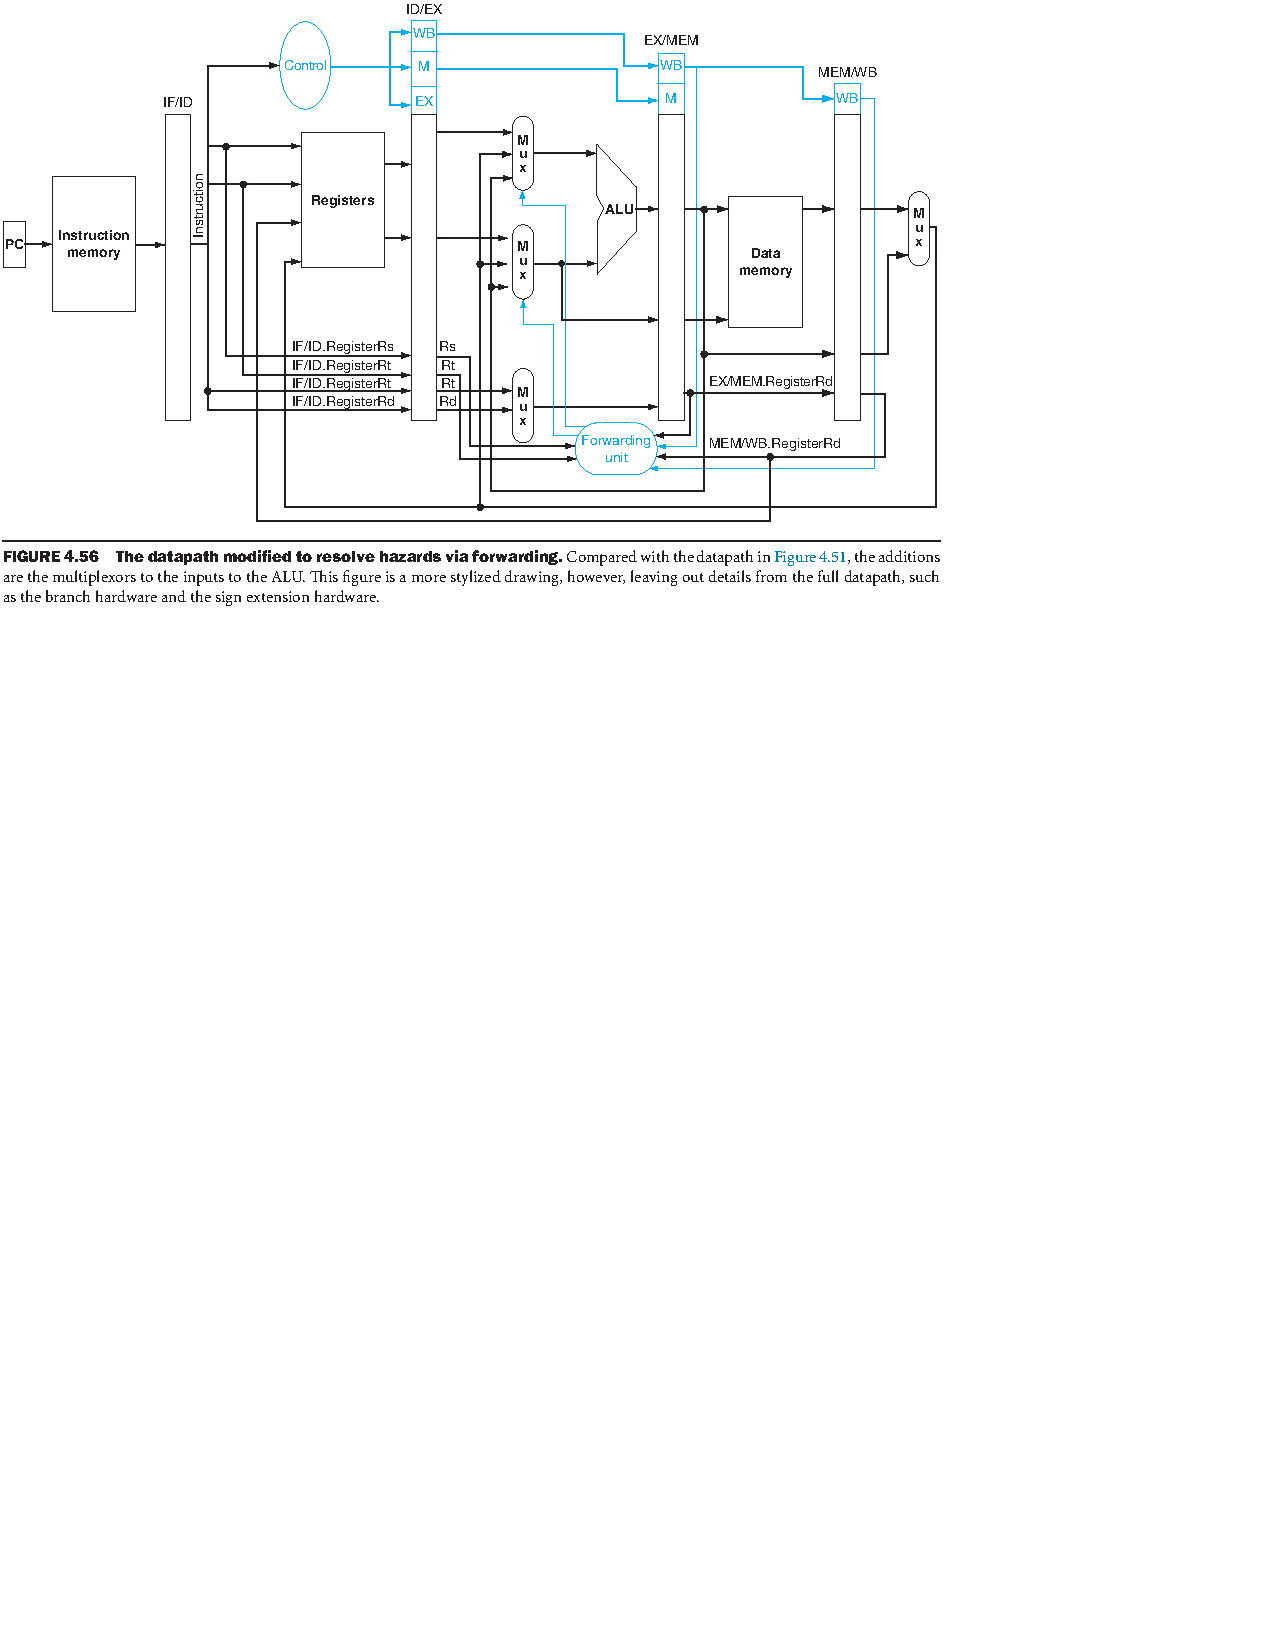
\includegraphics[width=\textwidth]{forwarding.pdf}

\begin{table}[h]
    \centering
    \begin{tabular}{>{\ttfamily}c>{\ttfamily}ll}
        \toprule
        多选器控制 & 源 & 解释 \\
        \midrule
        ForwardA=00 & ID & 第一个 ALU 操作数来自寄存器堆 \\
        ForwardA=10 & EX & 第一个 ALU 操作数由上一个 ALU 运算结果转发获得 \\
        ForwardA=01 & MEM & 第一个 ALU 操作数从数据存储器或者前面的 ALU 运算结果中转发获得 \\
        ForwardB=00 & ID & 第二个 ALU 操作数来自寄存器堆 \\
        ForwardB=10 & EX & 第二个 ALU 操作数由上一个 ALU 运算结果转发获得 \\
        ForwardB=01 & MEM & 第二个 ALU 操作数由数据存储器或者前面的 ALU 结果转发获得 \\
        \bottomrule
    \end{tabular}
\end{table}

EX 冒险:

\begin{verbatim}
    if (EX_REG_WRITE && 
        (EX_WRITE_REG != 0) && 
        (EX_WRITE_REG == ID_INST[25:21])) 
        ForwardA = 10;
    if (EX_REG_WRITE && 
        (EX_WRITE_REG != 0) && 
        (EX_WRITE_REG == ID_INST[20:16]))
        ForwardB = 10;
\end{verbatim}

MEM 冒险:

\begin{verbatim}
    if (MEM_REG_WRITE && (MEM_WRITE_REG != 0) 
        && !(EX_REG_WRITE && (EX_WRITE_REG != 0)
            && (EX_WRITE_REG != ID_INST[25:21]))
        && (MEM_WRITE_REG == ID_INST[25:21]))
        ForwardA = 01;
    if (MEM_REG_WRITE && (MEM_WRITE_REG != 0) 
        && !(EX_REG_WRITE && (EX_WRITE_REG != 0)
            && (EX_WRITE_REG != ID_INST[20:16]))
        && (MEM_WRITE_REG == ID_INST[20:16]))
        ForwardB = 01;
\end{verbatim}

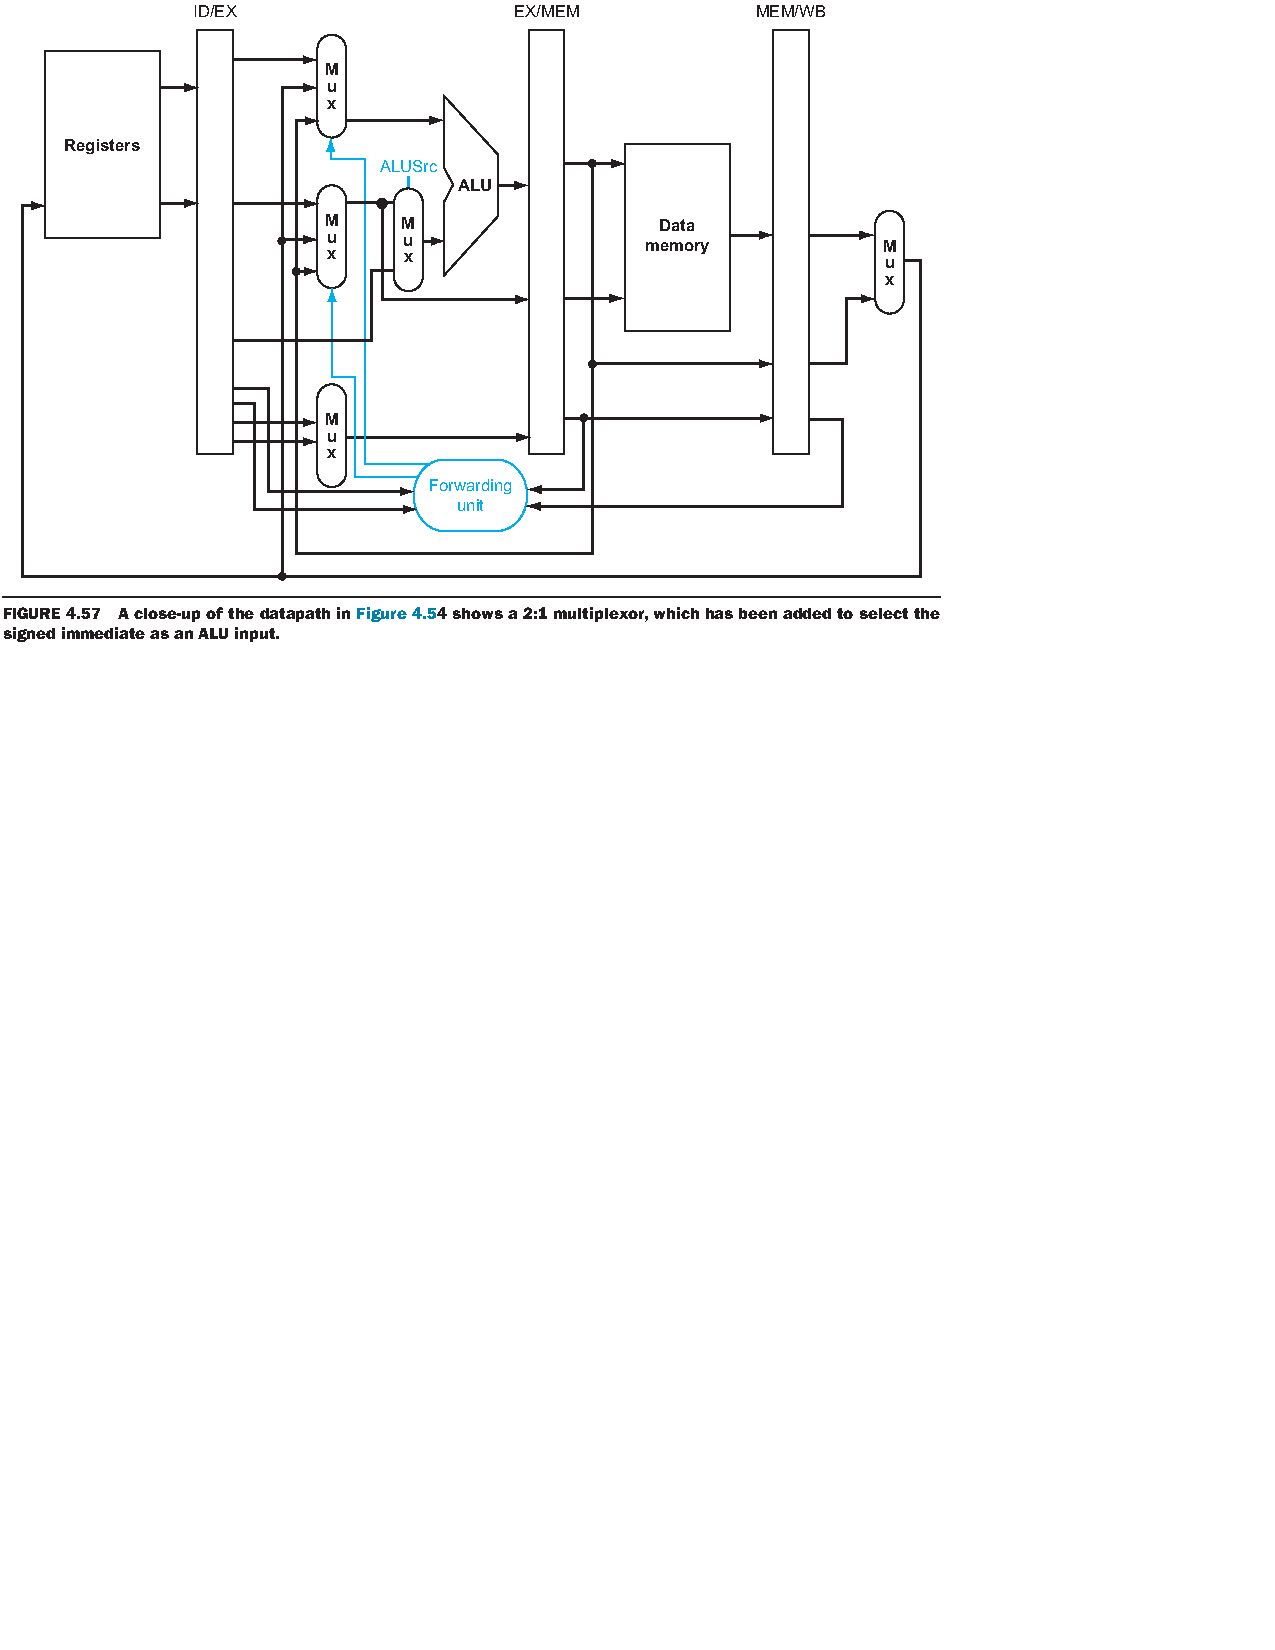
\includegraphics[width=\textwidth]{Imm.pdf}

\begin{verbatim}
    ALU alu(
        .input1(SHAMT ? ID_INST[10:6] : 
            (ForwardA == 2'b00 ? ID_READ_DATA1 :
                (ForwardA == 2'b10 ? EX_ALU_RES : 
                    WRITE_DATA_WB))
        ),
        .input2(ID_ALU_SRC ? ID_OPAND : 
            (ForwardB == 2'b00 ? ID_READ_DATA2 :
                (ForwardB == 2'b10 ? EX_ALU_RES :
                    WRITE_DATA_WB))
        ),
        .aluCtr(ALU_CTR),
        .zero(ZERO_EX),
        .aluRes(ALU_RES_EX)
    );
\end{verbatim}

\subsection{停顿机制}

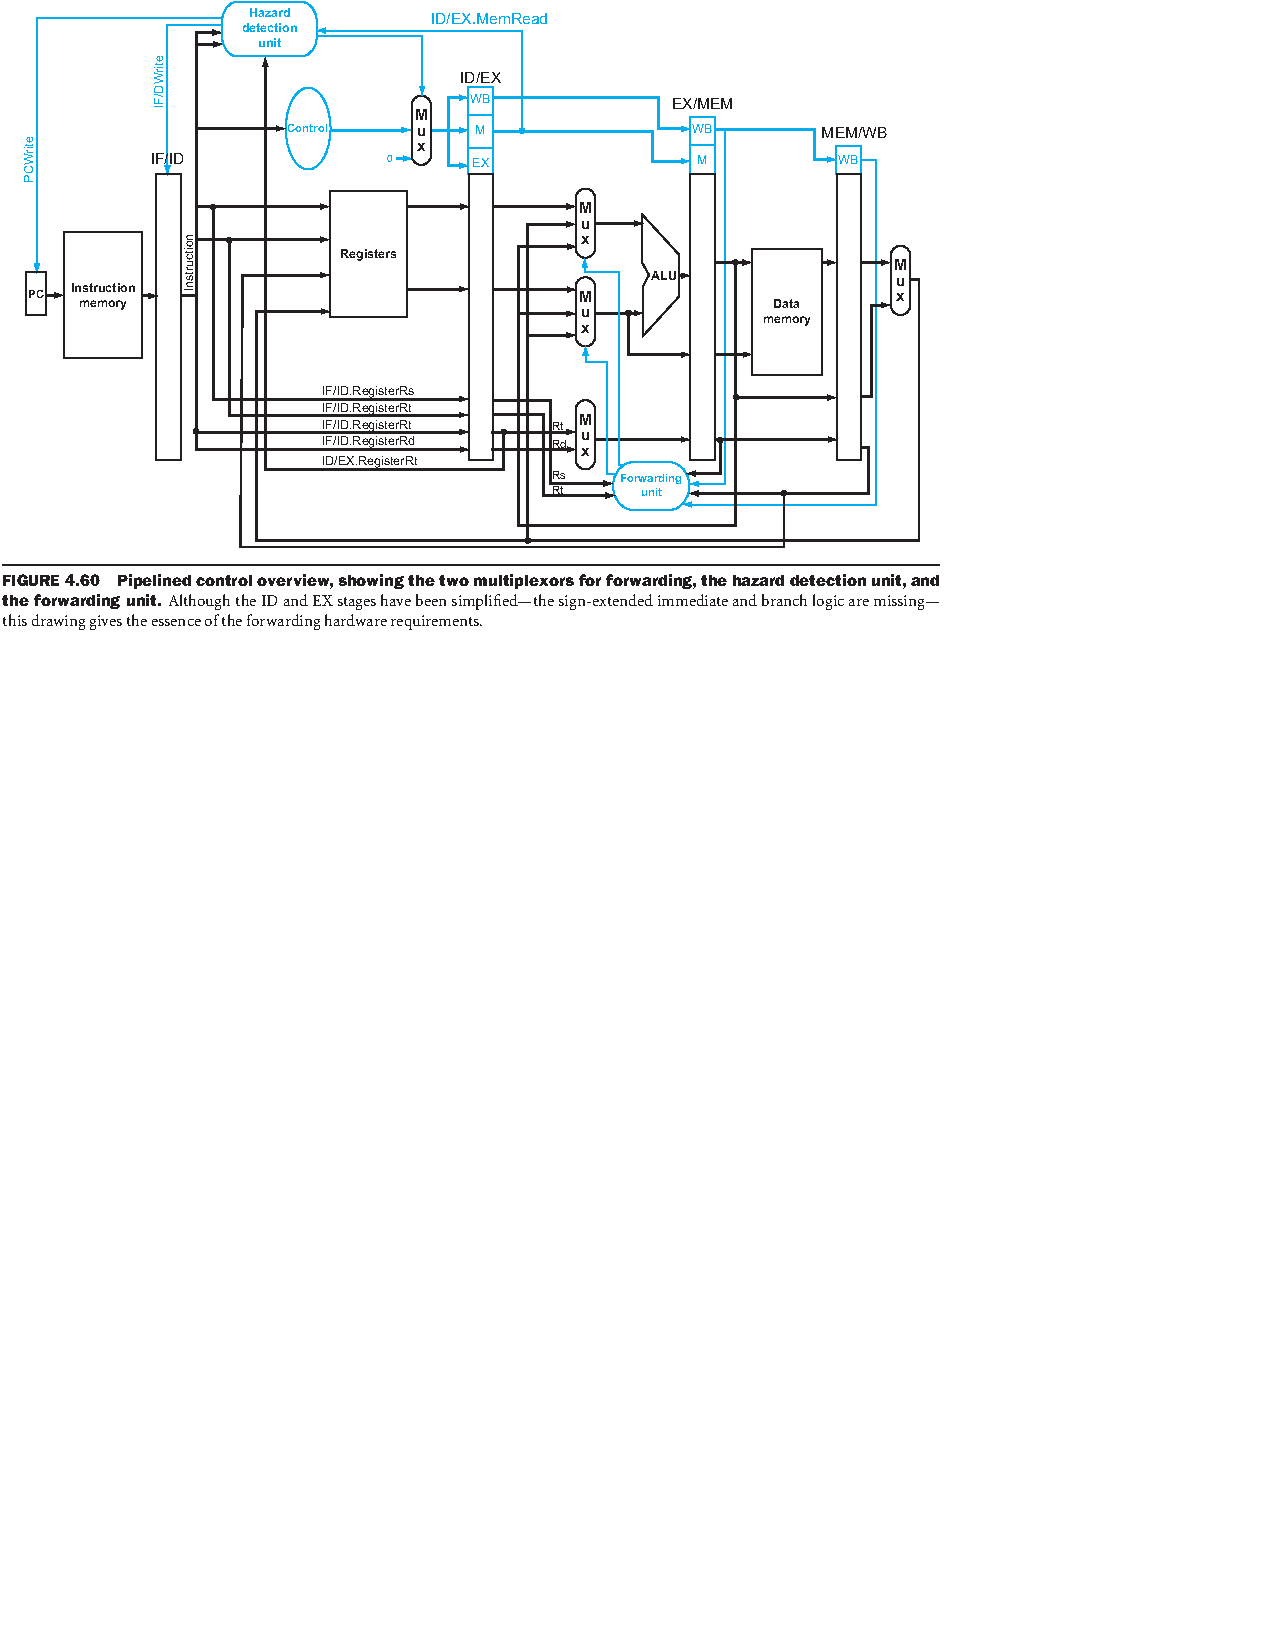
\includegraphics[width=\textwidth]{stall.pdf}

\begin{verbatim}
    wire stalling = (ID_MEM_READ && 
        ((ID_INST[20:16] == IF_INST[25:21]) 
        || (ID_INST[20:16] == IF_INST[20:16]))) ? 
            1 : 0;
\end{verbatim}

\subsection{预测不发生机制}

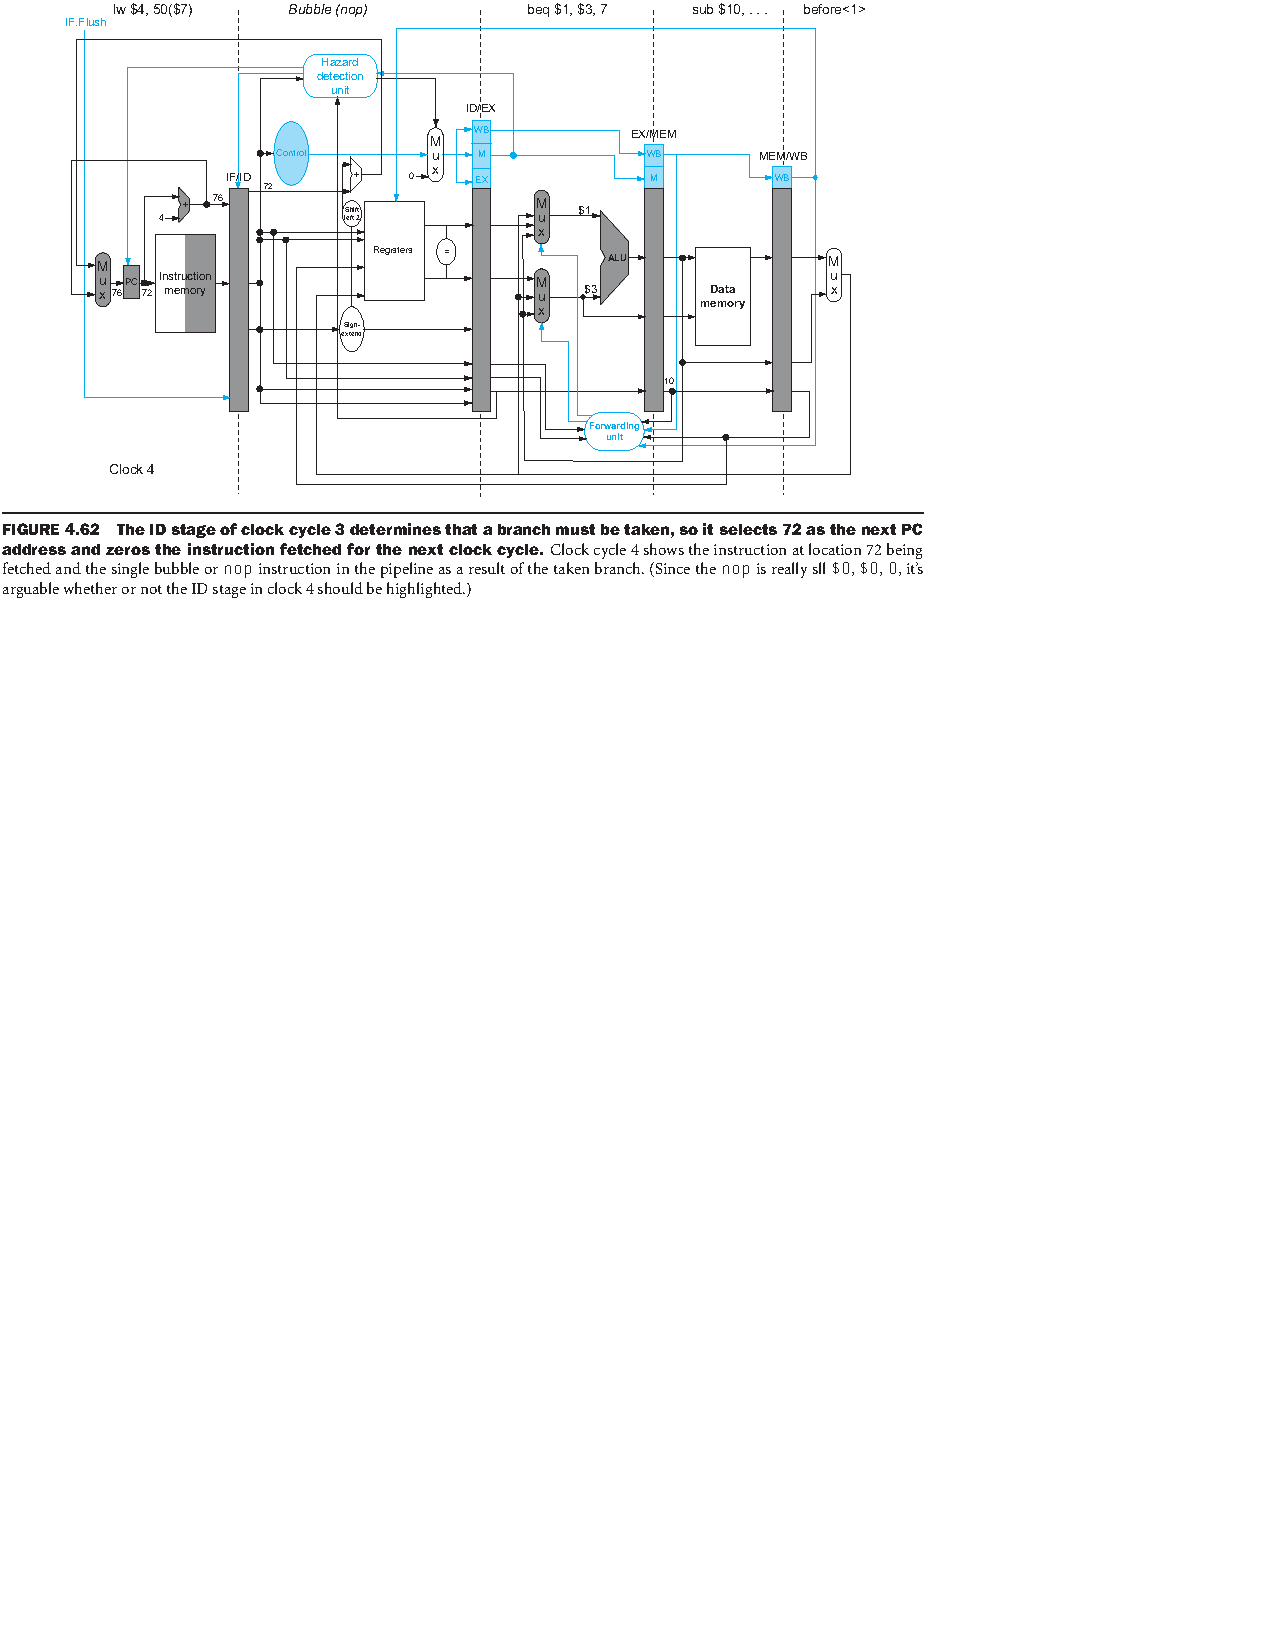
\includegraphics[width=\textwidth]{predict-not-taken.pdf}

将 branch 判定提前到 ID 段。

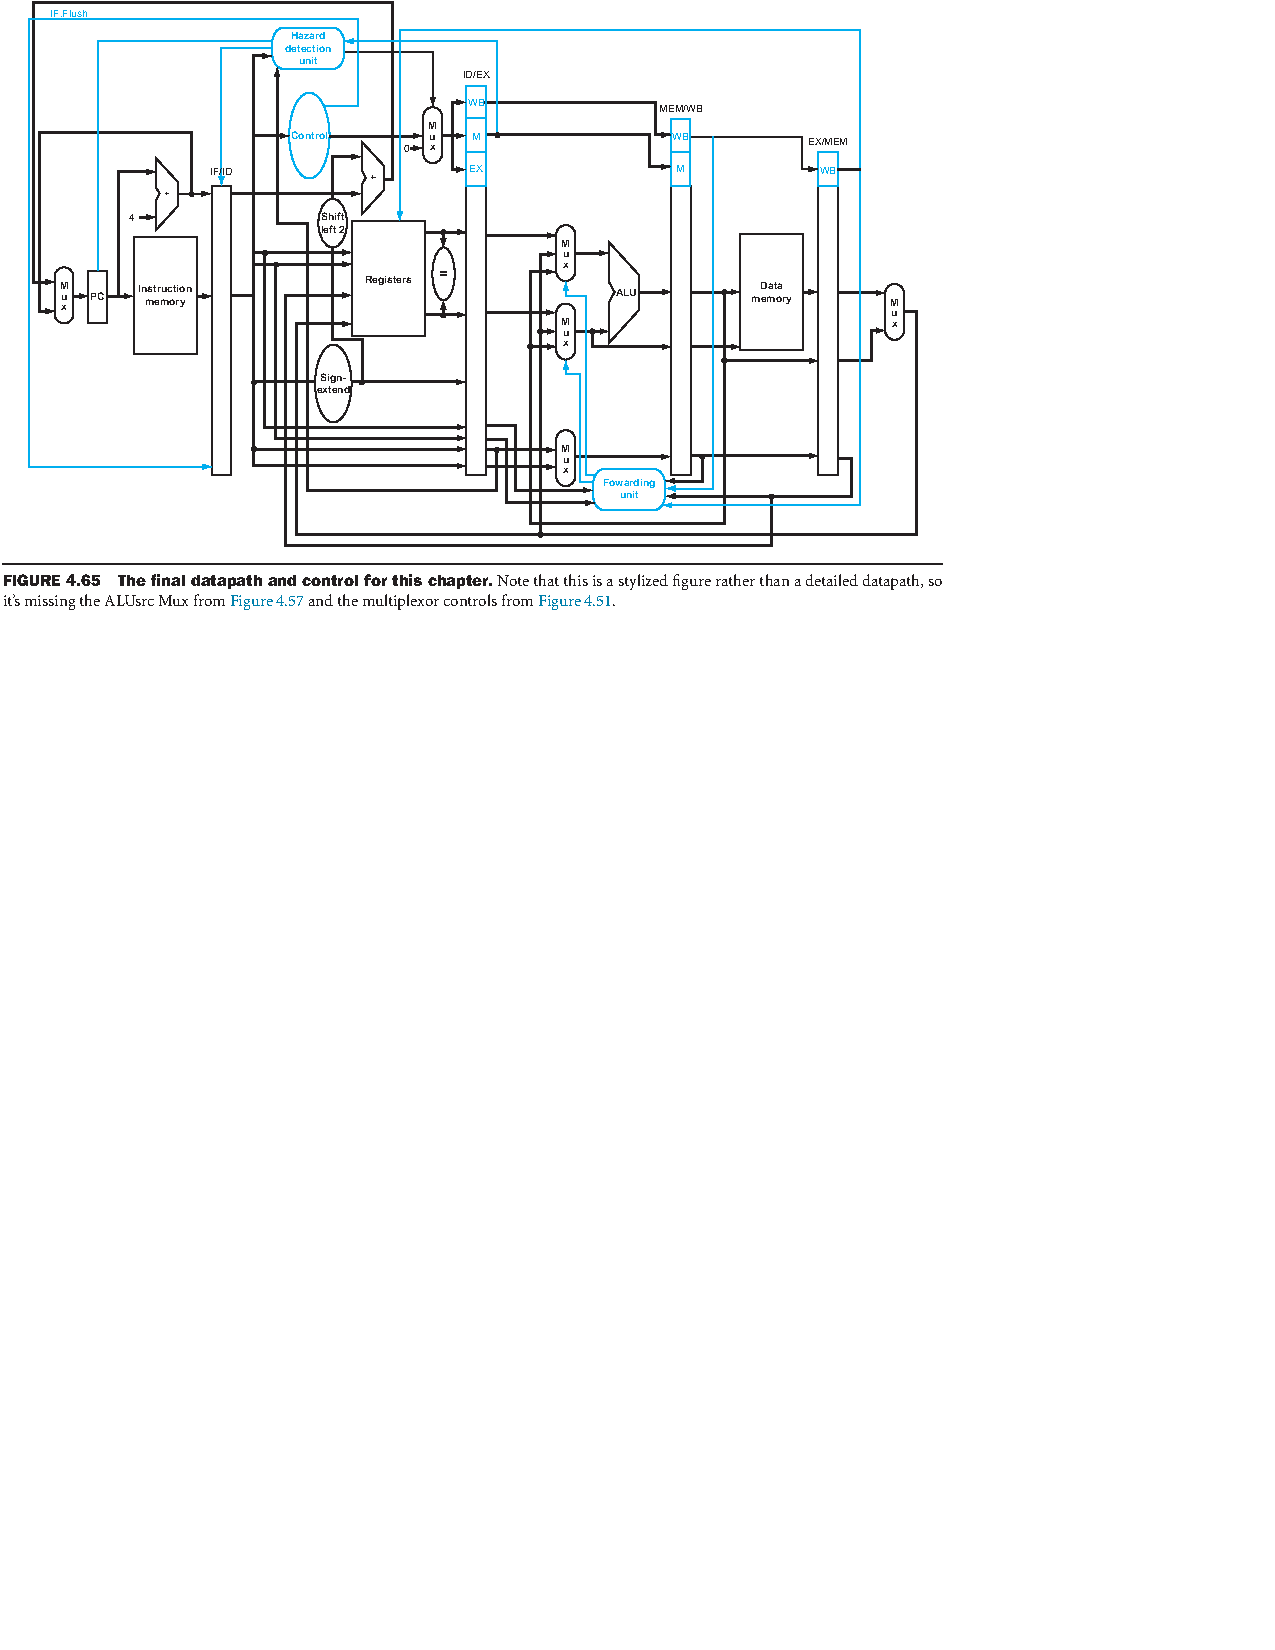
\includegraphics[width=\textwidth]{FINAL.pdf}

\section{仿真结果}



\section{实验心得}



\end{document}